\begin{pastexam}[label={px:ntu-109-bime-ds-04}]{臺大生機所 109 學年度 第 4 題}
（問答）

(20\%) Please write a pseudocode function that deletes a key (the input of the function) in a
\textbf{binary search tree (BST)}.

Note: A node in a \textbf{BST} has two pointers, named `left' and `right', respectively, where the
`left' pointer is used to find the left child of the node and the `right' pointer is used to find
the right child.
\end{pastexam}

\begin{pastsoln}
題目說節點只有 left、right 兩個指標，沒有父指標，所以用遞迴：函式回傳刪除之後這棵子樹的根，
呼叫的人把它接回去，就不必知道父節點是誰。 這是資結書虛擬碼~9.7 的寫法。

\textbf{三種情況}。 找到要刪的節點 $z$ 之後：
\begin{enumerate}
\item $z$ 沒有子節點：直接拿掉，父節點那一邊改成 \NIL。
\item $z$ 只有一個子節點：讓那個子節點頂上來，接到 $z$ 原本的位置。
\item $z$ 有兩個子節點：找 $z$ 的後繼 $s$（右子樹裡最小的節點），把 $s$ 的鍵（連同其他資料）複製
到 $z$，再到右子樹裡把 $s$ 刪掉。 $s$ 是右子樹最左邊的節點，沒有左子節點，刪它只會落在情況 1
或 2。 換上來的 $s.\mathit{key}$ 比左子樹所有的鍵大（它在 $z$ 的右子樹裡），又比右子樹剩下的鍵小
（它是右子樹最小的），BST 的性質保持住。
\end{enumerate}

\begin{pseudo}{刪除鍵值 $k$，回傳子樹新的根；呼叫方式 $\mathit{root} \gets \proc{Tree-Delete}(\mathit{root}, k)$}
\Function{Tree-Delete}{$x, k$}
    \If{$x = \NIL$}
        \State \Return \NIL \Comment{$k$ 不在樹裡}
    \EndIf
    \If{$k < x.\mathit{key}$}
        \State $x.\mathit{left} \gets \Call{Tree-Delete}{x.\mathit{left}, k}$
    \ElsIf{$k > x.\mathit{key}$}
        \State $x.\mathit{right} \gets \Call{Tree-Delete}{x.\mathit{right}, k}$
    \ElsIf{$x.\mathit{left} = \NIL$} \Comment{情況 1、2：沒有左子節點}
        \State \Return $x.\mathit{right}$
    \ElsIf{$x.\mathit{right} = \NIL$} \Comment{情況 2：只有左子節點}
        \State \Return $x.\mathit{left}$
    \Else \Comment{情況 3：兩個子節點}
        \State $s \gets x.\mathit{right}$
        \While{$s.\mathit{left} \ne \NIL$} \Comment{右子樹最左邊的節點是後繼}
            \State $s \gets s.\mathit{left}$
        \EndWhile
        \State $x.\mathit{key} \gets s.\mathit{key}$ \Comment{連同其他資料一起複製}
        \State $x.\mathit{right} \gets \Call{Tree-Delete}{x.\mathit{right}, s.\mathit{key}}$
    \EndIf
    \State \Return $x$
\EndFunction
\end{pseudo}

第 8 行同時處理情況 1 和「只有右子節點」的情況 2：沒有左子節點時，右子樹（可能是空的）頂
上來。 第 17 行到右子樹裡刪 $s.\mathit{key}$，那次遞迴會停在 $s$，而 $s$ 沒有左子節點，走第 8--9 行，
不會再進入情況 3。 被拿掉的節點在第 9、11 行回傳之後由呼叫的程式釋放（C 裡要先記下 $x$ 再
\texttt{free}）。

\textbf{例子}。 對下面左邊的樹刪除 $30$（情況 3）：$30$ 的右子樹最小的是 $35$，把 $35$ 複製到根，
再到右子樹刪掉原本的 $35$；它只有右子節點 $38$（情況 2），$38$ 頂上來。
\begin{center}
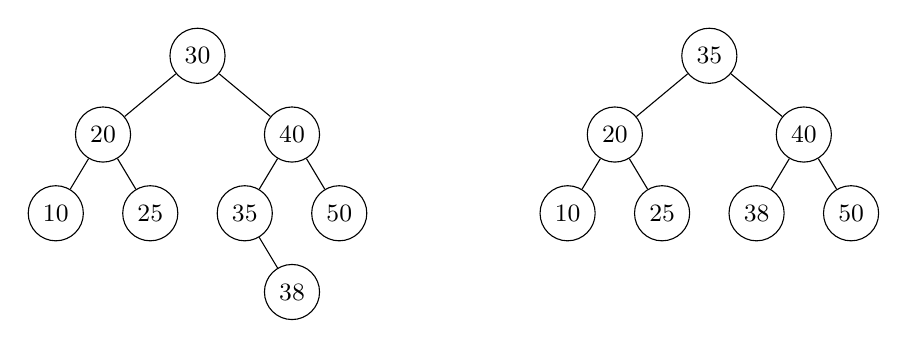
\begin{tikzpicture}[level distance=10mm,
  every node/.style={circle,draw,minimum size=7mm,inner sep=0pt,font=\small},
  level 1/.style={sibling distance=24mm}, level 2/.style={sibling distance=12mm}]
\node {30}
  child {node {20} child {node {10}} child {node {25}}}
  child {node {40} child {node {35} child[missing] child {node {38}}} child {node {50}}};
\begin{scope}[xshift=65mm]
\node {35}
  child {node {20} child {node {10}} child {node {25}}}
  child {node {40} child {node {38}} child {node {50}}};
\end{scope}
\end{tikzpicture}
\end{center}
刪除後中序走訪是 $10, 20, 25, 35, 38, 40, 50$，仍然遞增，是 BST。 若再刪 $25$（葉節點），是情況 1，
只要把 $20$ 的右指標改成 \NIL。

\textbf{時間}。 第 4--7 行沿著一條從根往下的路徑找 $k$；情況 3 再往下走到 $s$，第 17 行的遞迴走的也
是同一段路。 全部在一條根到葉的路徑上，時間 $O(h)$，$h$ 是樹高：平衡時 $O(\lg n)$，退化成一條鏈
時 $O(n)$。

\textbf{另一種寫法}：情況 3 也可以用前驅（左子樹最大的節點）代替後繼，結果是另一棵合法的 BST。
作答時寫清楚用哪一種即可。
\end{pastsoln}
